\documentclass[tikz,border=2pt]{standalone}
\usepackage{amsmath}
\usetikzlibrary{arrows.meta, decorations.pathreplacing}
\begin{document}
% Fibonacci, x_{t+2} = x_{t+1} + x_t: the k = 2 initial values x_0 = 0, x_1 = 1 fix the
% solution 0, 1, 1, 2, 3, 5, 8; each new term is computed from the two before it.
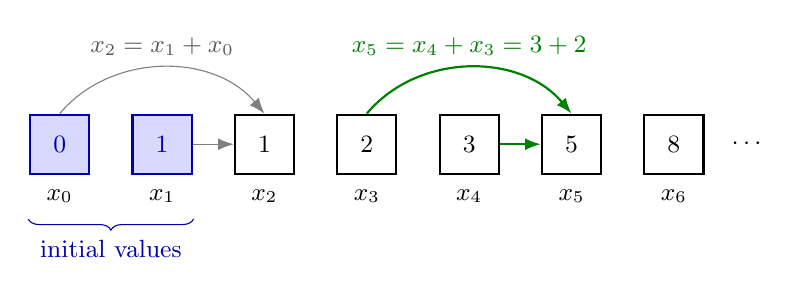
\begin{tikzpicture}[font=\small, >={Latex[length=2mm]}]
  \def\d{1.3}
  \foreach \v [count=\i from 0] in {0,1,1,2,3,5,8} {
    \ifnum\i<2
      \node[draw, thick, blue!70!black, fill=blue!15, minimum size=0.75cm] (x\i) at (\i*\d,0) {$\v$};
    \else
      \node[draw, thick, minimum size=0.75cm] (x\i) at (\i*\d,0) {$\v$};
    \fi
    \node[anchor=north] at (\i*\d,-0.45) {$x_{\i}$};
  }
  \node at (7*\d-0.35,0) {$\cdots$};
  % the first step (grey) and a later step (green) of the recursion
  \draw[->, gray] (x0.north) to[out=50, in=130] (x2.north);
  \draw[->, gray] (x1.east) -- (x2.west);
  \node[gray!70!black, anchor=south] at (1*\d,1.0) {$x_2=x_1+x_0$};
  \draw[->, green!50!black, thick] (x3.north) to[out=50, in=130] (x5.north);
  \draw[->, green!50!black, thick] (x4.east) -- (x5.west);
  \node[green!50!black, anchor=south] at (4*\d,1.0) {$x_5=x_4+x_3=3+2$};
  % initial values
  \draw[decorate, decoration={brace, mirror, amplitude=4pt}, blue!70!black]
    (-0.4,-0.95) -- (\d+0.4,-0.95)
    node[midway, below=4pt, align=center] {initial values};
\end{tikzpicture}
\end{document}
